\documentclass[10pt,twocolumn,letterpaper]{article}

\usepackage{cvpr2019AuthorKit/latex/cvpr}
\usepackage{times}
\usepackage{epsfig}
\usepackage{graphicx}
\usepackage{amsmath}
\usepackage{amssymb}
\usepackage{xcolor}
\usepackage{algorithm}
\usepackage{algorithmic}
\usepackage{multirow}
% \usepackage{arydshln}
\usepackage{subcaption}

\def\x{{\mathsf x}}

% Include other packages here, before hyperref.

% If you comment hyperref and then uncomment it, you should delete
% egpaper.aux before re-running latex.  (Or just hit 'q' on the first latex
% run, let it finish, and you should be clear).
\usepackage[breaklinks=true,bookmarks=false]{hyperref}

\cvprfinalcopy % *** Uncomment this line for the final submission

\def\cvprPaperID{****} % *** Enter the CVPR Paper ID here
\def\httilde{\mbox{\tt\raisebox{-.5ex}{\symbol{126}}}}

% Pages are numbered in submission mode, and unnumbered in camera-ready
%\ifcvprfinal\pagestyle{empty}\fi
\setcounter{page}{4321}


%% helper definitions
\def\eg{\emph{e.g.\hspace{0.3em}}}
\def\Eg{\emph{E.g.\hspace{0.3em}}}
\def\ie{\emph{i.e.\hspace{0.3em}}}
\def\etal{\emph{et al.\hspace{0.3em}}}

% TODO
\newcommand{\todo}[1]{}
\renewcommand{\todo}[1]{{\color{red} TODO: {#1}}}

\begin{document}

%%%%%%%%% TITLE
\title{Multi-Task Mutual Learning for Vehicle Re-Identification}

\author{Georgia Rajamanoharan\\
Vision Semantics Ltd\\
{\tt\small georgia@visionsemantics.com}
% For a paper whose authors are all at the same institution,
% omit the following lines up until the closing ``}''.
% Additional authors and addresses can be added with ``\and'',
% just like the second author.
% To save space, use either the email address or home page, not both
\and
Aytac Kanaci \hspace{0.7cm}
%Queen Mary University of London\\
%{\tt\small secondauthor@i2.org}
%\and
Minxian Li  \hspace{0.7cm}
%Queen Mary University of London\\
%{\tt\small secondauthor@i2.org}
%\and
Shaogang Gong\\
Queen Mary University of London\\
{\tt\small \{a.kanaci,m.li,s.gong\}@qmul.ac.uk }
}

\maketitle
%\thispagestyle{empty}

%%%%%%%%% ABSTRACT
\begin{abstract}

\end{abstract}

%%%%%%%%% BODY TEXT
\section{Introduction}

%%% Background and motivation
As the ubiquitousness of surveillance cameras capturing vehicle in transport in
cities and highways increase, the need for analyzing this visual data has
become an interest in computer vision. With the advent of autonomous driving
and smart city applications the need for accurately analyzing vehicles in these
scenarios with related computer vision tasks \ie detection, classification and
pose estimation as well as re-identification is ever-increasing.

Vehicle re-identification (re-ID) aims at searching a target vehicle
(identity) across non-overlapping camera views by image matching.  
Vehicle re-identification received less attention than person re-identification
which is been studied extensively \cite{gong2014re, Li2018Harmonious,
chen2017person}.\todo{add more citation}  

As a unique ID of a vehicle, license plate has been widely used for vehicle
re-ID. However, license plate recognition is quite sensitive to image quality,
camera view and occlusion. Furthermore, license plate may be removed,
altered even faked in some cases, making it unreliable to identify a vehicle
simply by its license plate. Therefore, vehicle re-ID by visual appearance is
of great practical value in real-world applications such as smart cities.

A related problem to vehicle re-identification is fine-grained vehicle model 
classification such as ``Audi A4 2014''\cite{yang2015compcars}.  
However, the granularity of vehicle re-identification task is much finer
since the ideal target is to search a specific vehicle rather than a model, in
which the image instances of the same vehicle (identity) forms a separate
class.
%%% Vehicle re-id challenges 
However,
vehicle re-id by visual appearance is a
challenging task due to the very similar appearance of different vehicle instances
of the same model type and color, and a significant visual appearance variation
of the same vehicle instance in different camera views. In other words
large intra-instance differences of the same vehicle in different cameras,
and subtle inter-instance differences between different vehicles in the same
view, considering thousands of vehicles in a large scale smart city setting is
the main challenge of vehicle re-ID. Moreover, unlike person re-id 
orientation of vehicles results in self occlusion and drastic visual geometry
changes where in person re-id visual geometry or texture of the person's
appearance (wear) will not change.
% re-ID problem. A human body is usually upright, thus the texture or color of
% his/her wear will not change severely in different views. Deploying the
% person re-ID methods for vehicles directly cannot obtain satisfactory
% performance.
% Due to the fact that vehicles are rigid objects, unlike people, the orientation
% of the vehicle can alter very predictably the appearance of in a particular
% viewpoint. 


% This area promises the potential for more flexible means for vehicle
% recognition and search than Automatic Number Plate Recognition (ANPR). 

% be found as an instance-level object search problem.


%%% matching probe gallery
Formally re-ID  aims to find
target images of the same identity in a large gallery set given a probe image. 
In order to match appearances of objects, firstly we need to obtain an
embedding for the objects. A
match is then performed by using a suitable distance metric expressing the
closeness of two objects in an embedding space. A good embedding should be
invariant to illumination, scale and viewpoint changes. 

%%% we use CNNs
Recently, Convolutional Neural Network (CNN) has achieved state-of-the-art
performance in various computer vision 
recognition tasks, such as large-scale image classification 
face recognition  and person re-ID.
With the supervision of a carefully designed objective loss, typically
cross-entropy and/or triplet loss
% contrastive loss or triplet loss
CNN can learn efficient feature embedding

%%% Datasets and SOTA
Influenced by the recent advancements on person re-id vehicle re-id has started
to gain increasing attention, 
and a number of vehicle databases and additional labeling are now available to
facilitate this research
 including 
 VeRi-776\cite{Liu2016icme-veri, Liu2016eccv_veri},
 VehicleID\cite{liu2016vehicleid} and VRIC\cite{kanaci2018vehicle} and methods
 specific to vehicle re-ID becoming more frequent in various venues
 \cite{wang2017orientation, Shen_2017_ICCV, Zhou2018VAMI}.  

%%% Our method:
\todo{Expand near submission}
In this paper we propose a new mutual learning based network architecture, that
aims to simultaneously learn a number of tasks, plus a consensus, to build an
improved representation for the purpose of vehicle re-identification.
% Second, we propose to leverage multi-task learning to gen- erate discriminative
% feature representation by the joint op- timization of group sensitive triplet
% loss and softmax loss, which can be well applied to accomplish large scale
% vehicle re-identification towards real applications.

\section{Related Work}

\begin{figure*}
  \begin{subfigure}{.6\textwidth}
    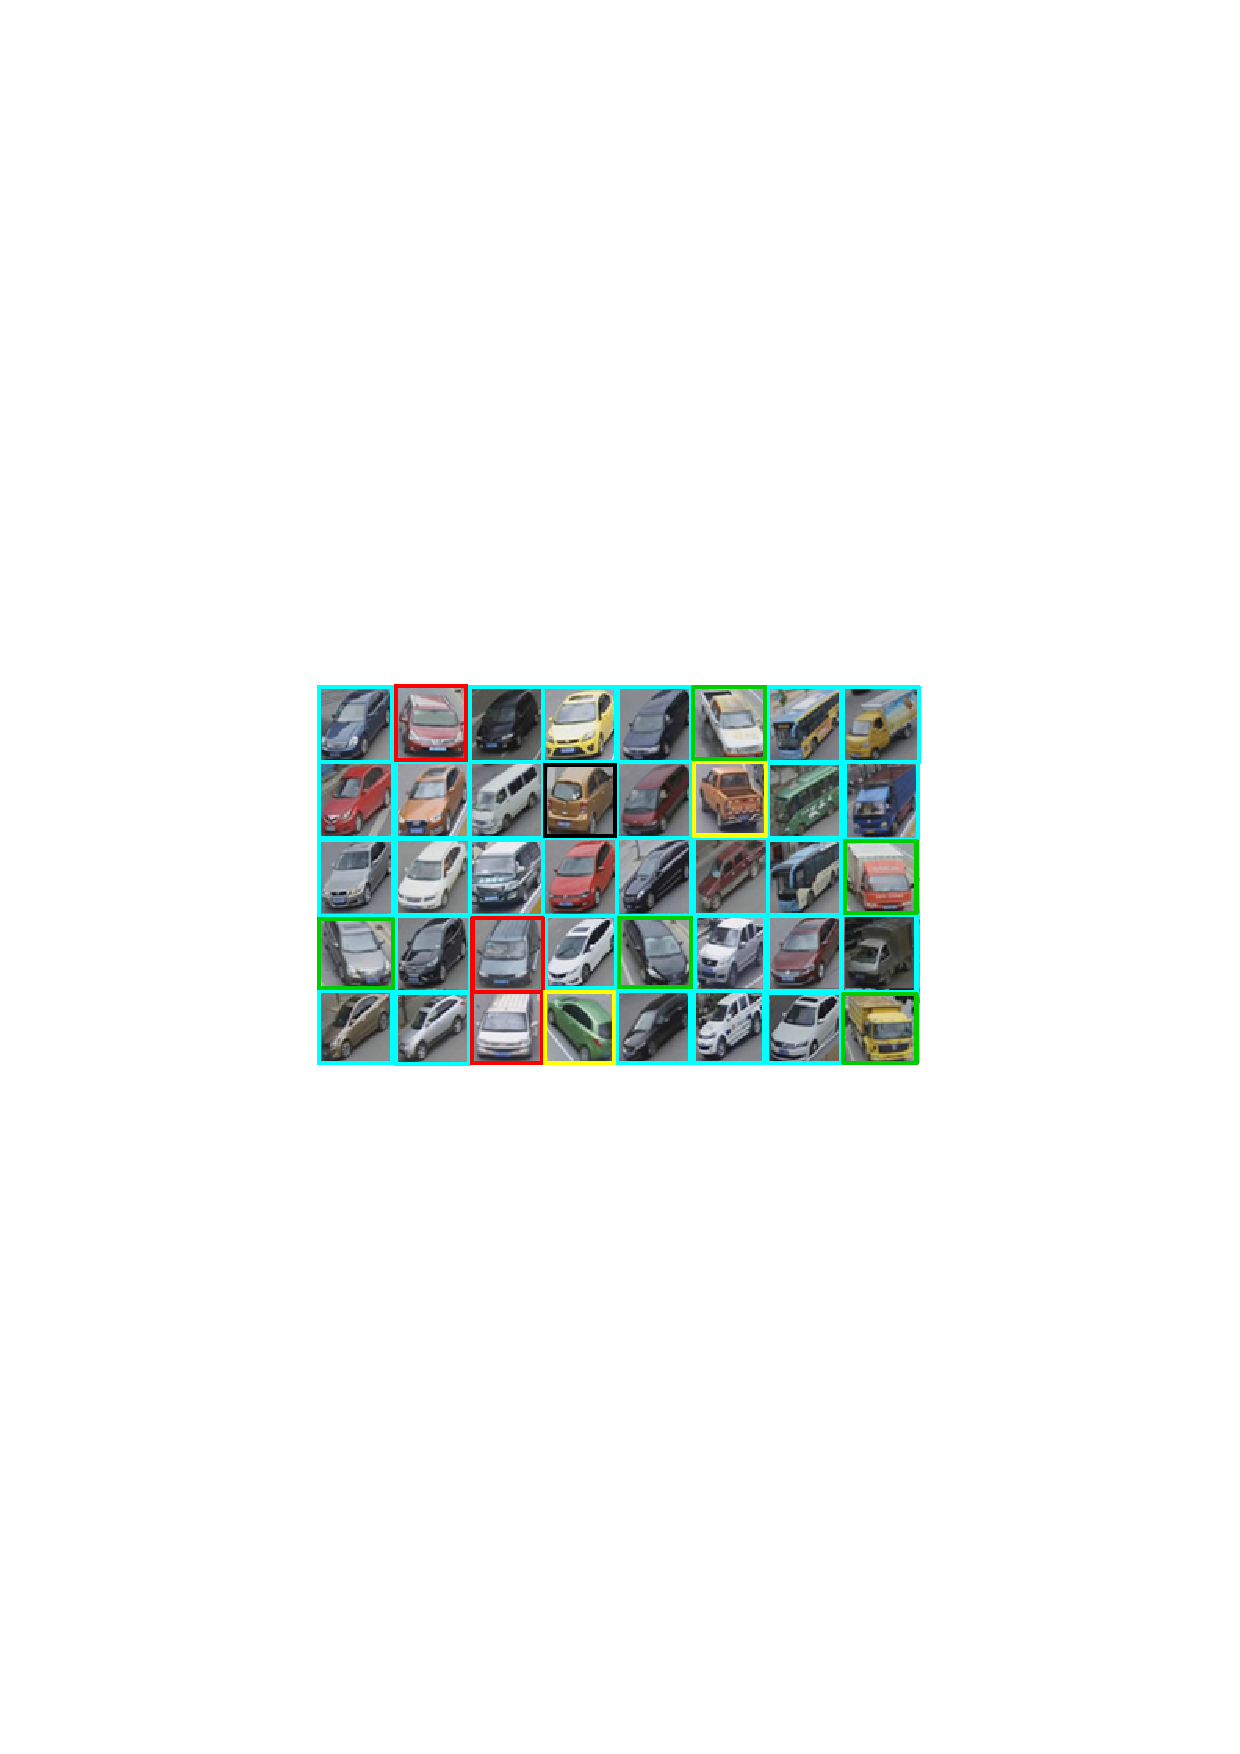
\includegraphics[width=\linewidth,trim=5cm 11cm 5cm 11cm,clip=true]{images/veri_orients.pdf}
  \end{subfigure}
  \begin{subfigure}{.4\textwidth}
    \centering
    \begin{tabular}{c | c | c}
      \hline
      Index & Orientation & Colour \\
      \hline
      0 & front & \textcolor{red}{red} \\
      1 & rear & \textcolor{blue}{blue}  \\
      2 & left  & - \\
      3 & left front & \textcolor{cyan}{cyan}  \\
      4 & left rear & \textcolor{yellow}{yellow}  \\
      5 & right  & - \\
      6 & right front & \textcolor{green}{green} \\
      7 & right rear & \textcolor{black}{black} \\
      \hline
    \end{tabular}
  \end{subfigure}
  \caption{Examples from the VeRi776 dataset with the orientation labels provided in \cite{wang2017orientation} (best viewed in colour).}
  \label{T:veri_veh_orientations}
\end{figure*}

\section{Multi-modal Vehicle Re-identification}

In order to perform Re-ID of previously unseen query vehicles, the aim of our model is to learn a feature embedding that allows for accurate retrivals based on distance (\eg L1) from the query image representation. In order to perform this task, we utilise training data containing a number of different labels: identity class labels as well as vehicle orientation class labels.
%and landmark position labels for a number of specific keypoints
We assume two sets of training examples $\mathcal{I}_1 = \{\mathbf{I_i}\}_{i=1}^N$ and $\mathcal{I}_2 = \{\mathbf{I_i}\}_{i=1}^M$, containing $N$ and $M$ training images respectively. Both training sets contain the associated identity class labels $\mathcal{Y}_1=\{y_i\}_{i=1}^N$ and $\mathcal{Y}_2=\{y_i\}_{i=1}^M$, where $y_i \in \left[1,...,N_{id}\right]$ for $N_{id}$ distinct vehicle idenities spanning the two training sets. However, in addition, $\mathcal{I}_1$ also contains orientation labels, $\mathcal{O_1}=\{o_i\}_{i=1}^N$, where $o_i \in \left[1,...,N_O\right]$ is the orientation (for $N_O$ possible orientations).
%and landmark position labels $\mathcal{L_1}=\{\mathbf{l_i}\}_{i=1}^N$ $\mathbf{l_i}=\{\left(x_{i,1},y_{i,1}\right),...,\left(x_{i,L},y_{i,L}\right)\}$ defines the position of $N_L$ keypoint landmarks for the vehicle within image $\mathbf{I}_i$, which we normalise according to the image size so that $x,y \in [0,1]$

In order to perform accurate re-ID, we use this data to build a model constructed from a number of branches, each of which is tasked with learning a specific aspect of the data concurrently. The branches of the model are as follows: A) Identity classification B) Identity classification from a scaled image C) Identity from grayscale image D) Identity plus the vehicles' orienations. The individual branches then form a consensus prediction on the identity of the training examples, and this consensus is then employed for regulation of the individual branches.
>>>>>>> e5e018ecb6db264c0f87b6bfce9aaf7c51b0ff67

\subsection{Model Structure and Feature Learning}

\begin{figure*}
  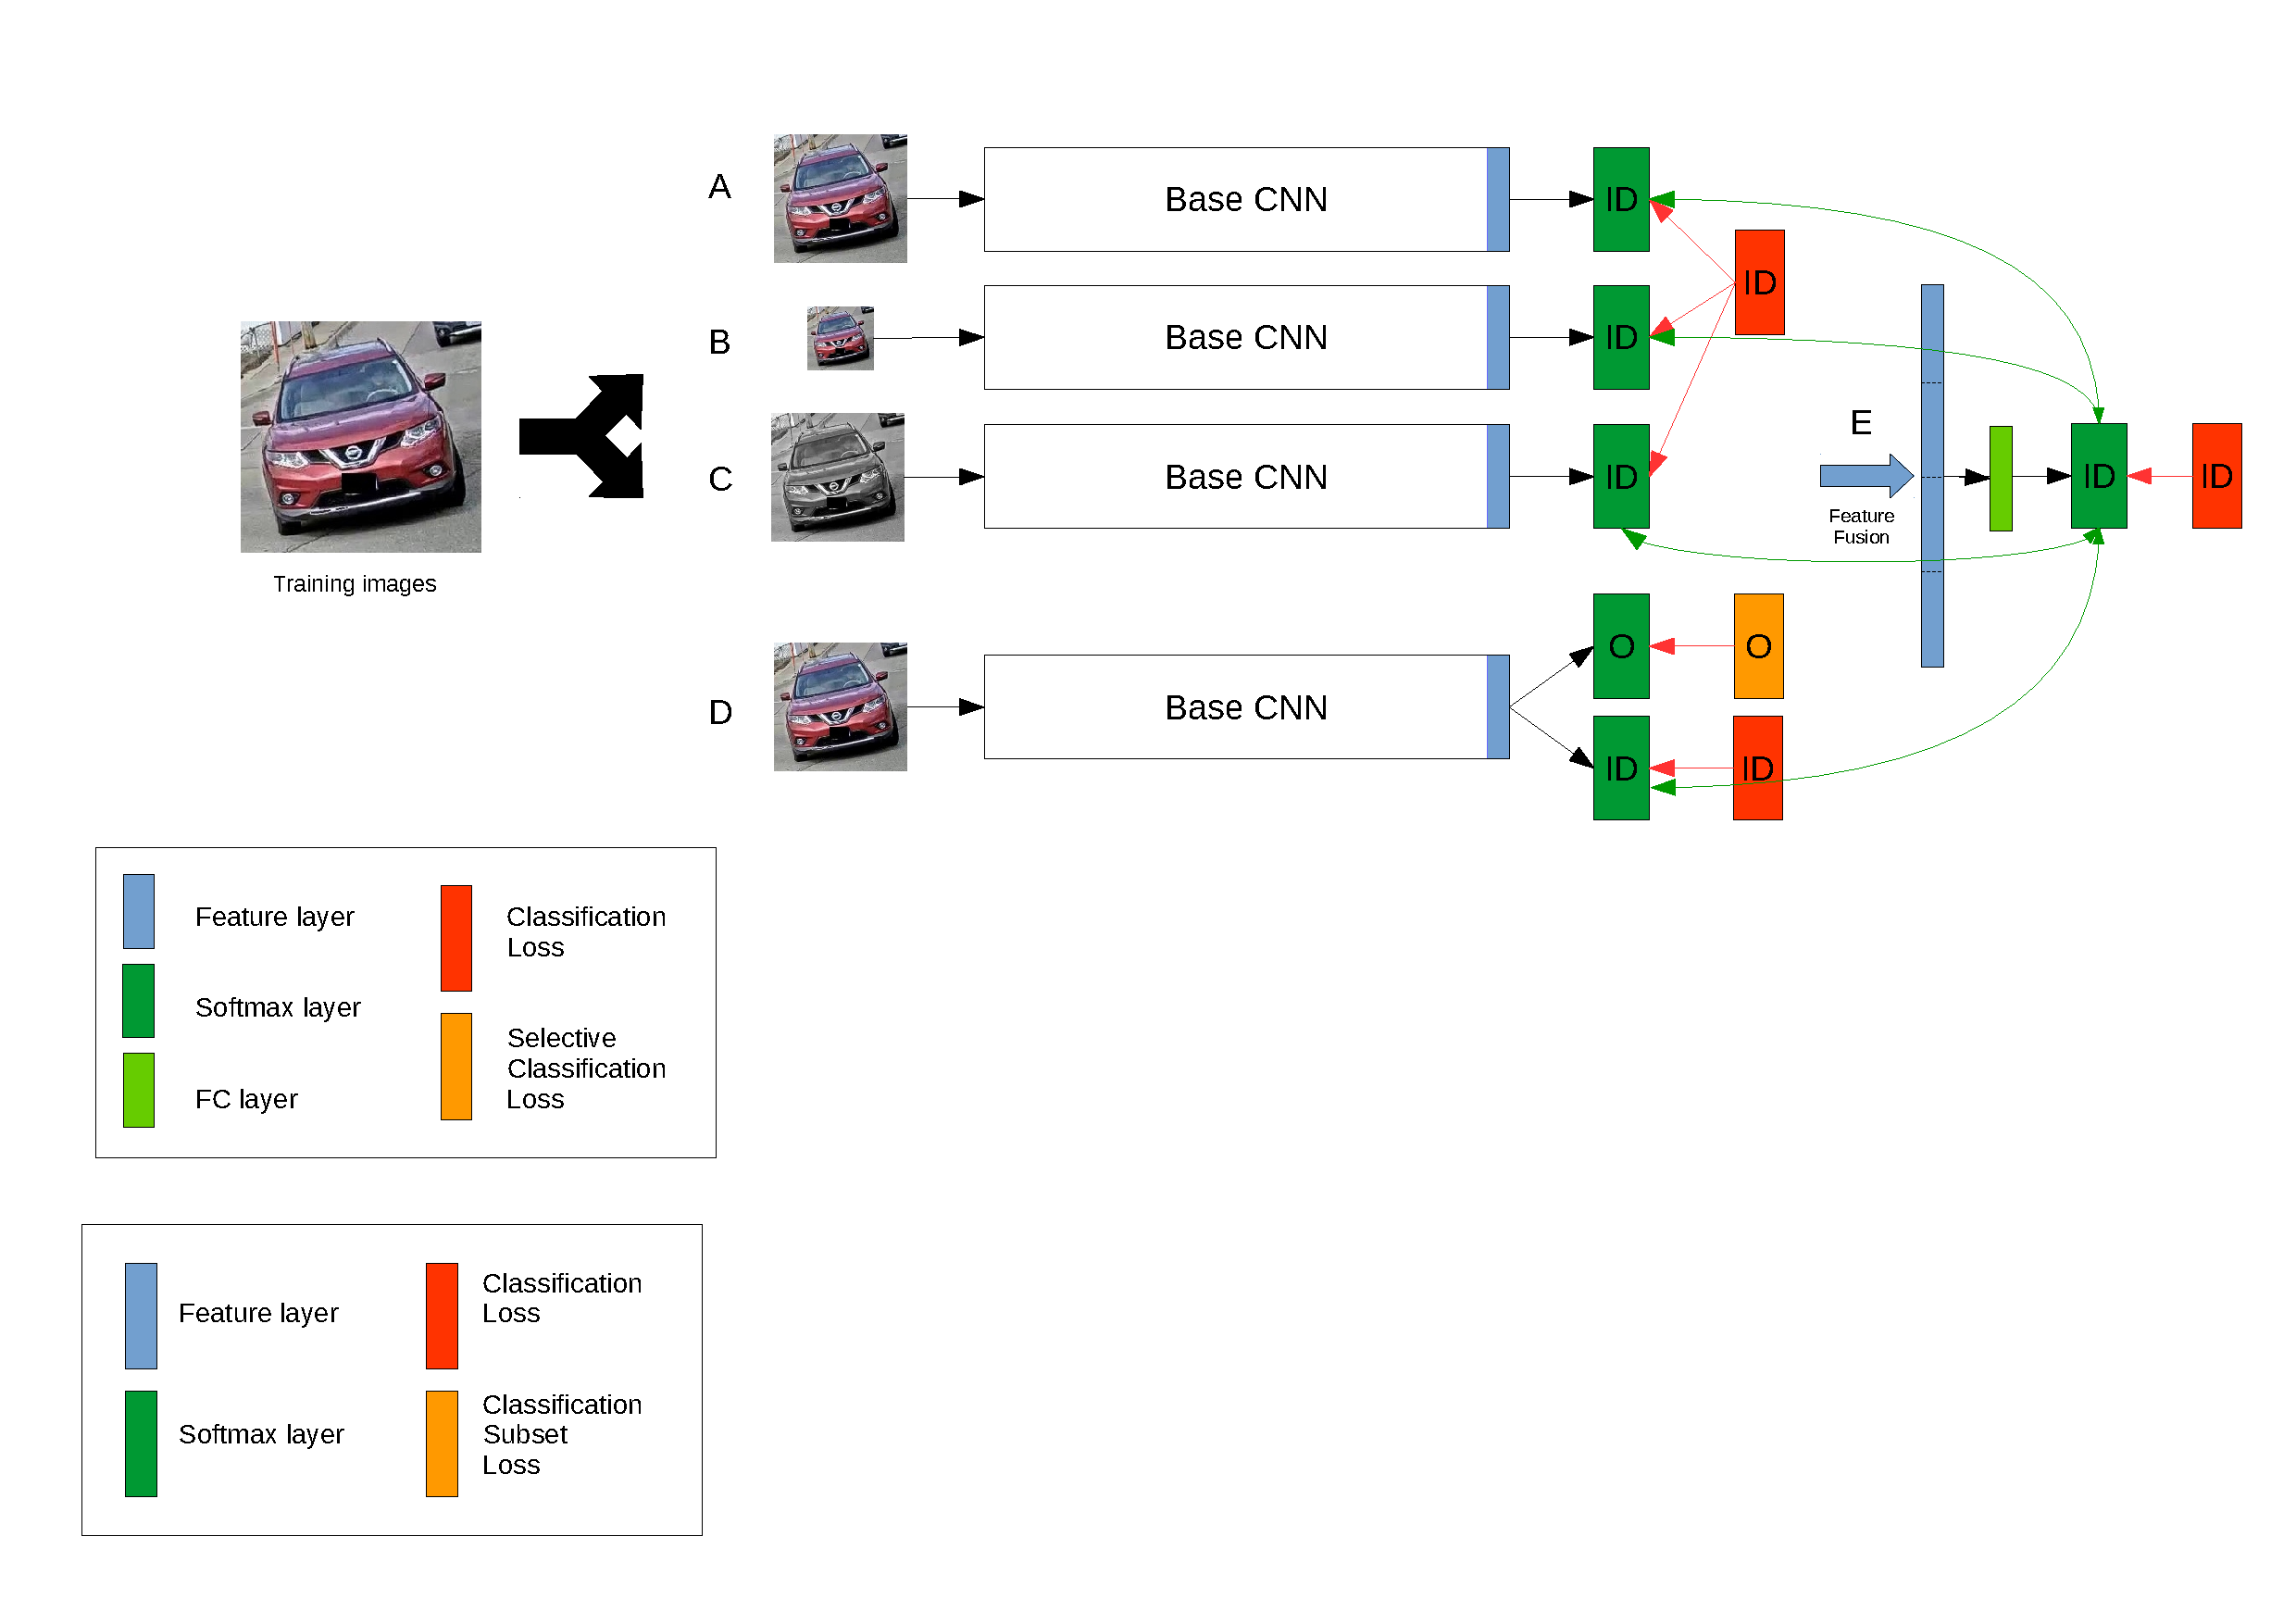
\includegraphics[width=\linewidth,trim=0cm 8cm 0cm 0cm,clip=true]{images/system_overview_orient_only.pdf}
  \caption{An overview of our proposed model (best viewed in colour). (A) Vehicle identity branch (B) Multi-scale analysis branch (C) Grayscale analysis branch (D) Vehicle orientation branch
    %(E) Vehicle landmark localisation branch.
(E) Consensus learning through feature fusion. Feedforward signals shown in black. Hard target (groundtruth) loss propagation shown in \textcolor{red}{red}. Soft target consensus feedback loss propagation shown in \textcolor{green}{green}.}
  \label{F:overview}
\end{figure*}

An overview of our proposed model can be seen in Figure \ref{F:overview}. The model is composed of a number of sub-branches, each of which is simultaneously learning a representation to solve its own set of tasks. In addition, there is a single fusion branch, which allows feature selection to be performed from the entire collection of individual representations. It is the output from this branch that is taken during deployment. Each sub-branch will now be described in more detail.

\paragraph{(A) Vehicle Identity}

The root branch of our model is tasked with learning the best representation for vehicle identity discrimination, for both training sets. Here, we exploit the cross entropy classification loss function in order to train one branch to predict vehicle identity. Thus the branch calculates the softmax posterior probability of the class label $y_i$ for a given training image $\mathbf{I_i}$:
\begin{equation}
  p_i^{ID} = p(\hat{y_i} = y_i|\mathbf{I_i}) = \frac{\exp(\hat{y_i})}{\sum_{k=1}^{N_{id}}\exp(\hat{y_k})}
  \label{E:softmax_id}
\end{equation}
where $\hat{y_k} = \mathbf{w_k^Tx_i}$, $\mathbf{x_i}$ is the feature vector for image $\mathbf{I_i}$ given by final layer of the branch, and $\mathbf{w_k}$ is the prediction function parameter for identity class $\emph{k}$. The loss across a minibatch of $N_B$ images can then be computed as:
\begin{equation}
  l_{ID} = -\frac{1}{N_B} \sum_{i=1}^{N_B} \log{p_i^{ID}}
  \label{E:cross_entropy_loss}
\end{equation}

\paragraph{(B) Multi-scale Analysis}

Here we exploit the multi-scale analysis that has previously been shown to be of benefit for the task of re-identification, both for persons \cite{chen2017person} and vehicles \cite{kanaci2018vehicle}. This is done by including a branch that is trained via cross entropy loss (Eq. \ref{E:cross_entropy_loss}) to predict the class identity from a rescaled version of the input image, in a similar way to branch A.

\paragraph{(C) Identity from Grayscale Image}

In order to encourage the model to focus on details of the vehicles, that allow for separation of highly similar identity classes, we ensure that one branch will be unable to use colour information for distinguishing between these classes. This is simply done by giving as input only the grayscale image, and again training the branch to predict identity via the cross entropy loss.

\paragraph{(D) Vehicle Orientation}

This branch is tasked with learning a representation to simultaneously predict the identity class and the orientation class, for examples for which this is known.
%In the case where the training images do not have associated orientation labels, this branch is trained in exactly the same way as the Vehicle Identity branch outlined above.
Both sets of labels are simultaneously employed in a joint loss function in order to optimise the branch for prediction of both identity and orientation. As orientation labels are not available for all training data, we employ a selective classifcation subset loss function, that allows the loss to be calculated across only the subset of the batch for which orientation labels are known.

Again, the cross entropy loss is exploited for this task. Hence, the branch calculates both Eq. (\ref{E:softmax_id}), as well as the softmax posterior probability of the orientation label $o_i$ for the images for which the orientation class is known:
\begin{equation}
  p_i^{O} = p(\hat{o_i} = o_i|\mathbf{I_i}) = \frac{\exp(\hat{o_i})}{\sum_{j=1}^{N_{O}}\exp(\hat{o_j})}
\end{equation}
where this time $\hat{o_j} = \mathbf{w_j^Tx_j}$, and $\mathbf{w_j}$ is the prediction function parameter for orientation class $\emph{j}$.

The loss for this branch is then calculated across the minibatch of images as:
\begin{equation}
  l_{O} = -\frac{1}{N_B} \sum_{i=1}^{N_B}\log{p_i^{ID}} + \frac{1}{N_S} \sum_{i=1}^{N_B}q_i^O
\end{equation}
where $N_S$ is the size of the subset of the minibatch for which orientation labels are known, and
\[
q_i^O =
\begin{cases}
    \log{p_i^{O}} & \text{if } o_i \in \mathcal{O} \\
    0 & \text{otherwise}
\end{cases}
\]
%% \paragraph{(E) Vehicle Landmark Localisation}

%% Vehicle landmarks are distinguishing features that must be employed in order to perform correct  re-identification of vehicles that look very similar. Hence it is crucial that our model picks up on these in its feature representation. In order to attempt to ensure this, we task one branch with simultaneously predicting the position of these landmarks (if present) as well as the identity class. As above, if no landmark labels are available in the minibatch, this branch is trained in exactly the same way as branch A.

%% If landmark groundtruth labels are available, these are employed to train the branch to predict the location of the landmarks which are present, while at the same time predict identity. As a different set of landmarks are visible, depending on the orientation of the vehicle, we need to take the absence of landmarks altogether into account when training this branch. Thus, we design a loss function that only penalises the predictions for landmarks that are present in the groundtruth labels for the minibatch examples. As this is the regression problem, we also set the final layer of the branch to output with linear activation, and take the Mean Squared Error (MSE) as the basis for our custom loss function. If the landmarks were all present in every training image, we could use the standard MSE loss:
%% \begin{equation}
%%   M = \frac{1}{N_B} \sum_{j=1}^{N_L} \sum_{i=1}^{N_B} (\hat{x_{i,j}} - x_{i,j})^2 + (\hat{y_{i,j}} - y_{i,j})^2
%% \end{equation}
%% where $\hat{x_{i,j}}$ and $\hat{y_{i,j}}$ are the predicted normalised coordinates. However, we need to alter this to remove landmarks that are not present at all in the image. Hence we design a selective MSE function that only takes into account those landmarks which the groundtruth labels indicate are present in the image. Thus:
%% \begin{equation}
%%   M = \sum_{j=1}^{N_L} \frac{1}{N_{B_j}} \sum_{i \in B_j} (\hat{x_{i,j}} - x_{i,j})^2 + (\hat{y_{i,j}} - y_{i,j})^2
%% \end{equation}
%% where $B_j$ is the subset of the minibatch examples for which landmark $j$ is present in image $\mathbf{I_i}$. Due to the nature of the landmarks, we can assume that there will be a similar number of examples in the batch that contain each landmark, hence we can approximate this as:
%% \begin{equation}
%%   M = \frac{1}{\bar{N_{B_j}}} \sum_{j=1}^{N_L}  \sum_{i \in B_j} (\hat{x_{i,j}} - x_{i,j})^2 + (\hat{y_{i,j}} - y_{i,j})^2
%% \end{equation}
%% where $\bar{N_{B_j}}$ is the mean number of examples containing each landmark, in order to simplify the calculation. Then the full loss function for the landmark branch becomes:
%% \begin{equation}
%%   l_{LM} = M - \frac{1}{N_B} \sum_{i=1}^{N_B} \log{p_i}
%% \end{equation}

\paragraph{(E) Consensus Learning and Feedback}

In order to harness the benefit of all branches for the purpose of vehicle re-identification, we employ consensus learning as proposed in \cite{chen2017person} and previously harnessed for vehicle re-id in \cite{kanaci2018vehicle}. This is done via feature fusion of the final convolutional feature maps from all branches for consensus learning. As our branches are based on the ResNet50 architecture, these feature maps are formed via an average pooling operation which result in feature vectors of length $2048$. Hence our fused features are of length $8192$. We then add one additional fully connected layer, of size $1024$, and the output of this passed to a final identity softmax classification layer, again employed with cross entropy loss. Hence:
\begin{equation}
  p_i^C = p(\hat{y_i^C} = y_i|\mathbf{I_i}) = \frac{\exp(\hat{y_i^C})}{\sum_{k=1}^{N_{id}}\exp(\hat{y_k^C})}
\end{equation}

Additionally, we also utilise a consensus propagation mechanism, similar to the previously proposed method \cite{chen2017person,kanaci2018vehicle}. Here the consensus output is taken as 'soft targets' (as opposed to the groundtruth label 'hard targets') for the training data, and used to feedback information about the predictions made by the entire ensemble of branches. This is done concurrently with the training of the individual branches. Thie method is inspired by the idea of Knowledge Distillation (KD) \cite{hinton2015distilling}, but is different in that here we employ the combined predictions from all the `student' branches as a \emph{virtual} teacher model, rather than utilising a pre-trainined powerful teacher model to provide the soft targets.

Specifically, the feedback mechanism employs the consensus probability predictions $P^C_i = \left[p_{i,1}^C,...,p_{i,j}^C,...,p_{i,N_{ID}}^C\right]$ given image $\mathbf{I_i}$, feeding these into the cross entropy loss between the two distributions to provide a consensus regularisation loss for the branch:
\begin{equation}
  \mathcal{H}_i = \mathcal{H}(P^C_i, P_i) = -\frac{1}{N_{ID}}\sum_{j=1}^{N_{ID}} p_j^c \log{p_j}
\end{equation}
The total consensus loss for a particular branch is then:
\begin{equation}
  l_{C} = \frac{1}{N_B} \sum_{i=1}^{N_B} \mathcal{H}_i
\end{equation}
This is added to each individual branch's loss functions. In addition, this mechanism provides regularisation of the whole network by propagating all of the consensus losses back through the feature fusion layer, which also boosts the learning of the ensemble.

\subsection{Model Training}

In order to train our model, we combine both training sets, $\mathcal{I}_1$ and $\mathcal{I}_2$, and employ batches that contain both images with and without orientation labelling. The full training algorithm can be seen in Algorithm \ref{A:model_training}.

\begin{algorithm}[t]
  \begin{algorithmic}
    \REQUIRE{Training sets $\mathcal{I}_1$ $\mathcal{I}_2$, labels $\mathcal{Y}_1$ $\mathcal{Y}_2$\
      $\mathcal{O}_1$, model $\mathcal{M}$}
    \STATE{$\bullet$ Initialise network branches with pre-trained ImageNet weights}
    \STATE{$\bullet$ Initialise output layers of $\mathcal{M}$ randomly}

    \FOR{epoch $e \in (1, E)$}

        \STATE{$\bullet$ Feed-forward through model to obtain all branch identity classification \
          predictions on images in $\mathcal{I}_1$ and $\mathcal{I}_2$}
        \STATE{$\bullet$ Feed-forward to obtain orientation classification predictions on $\mathcal{I}_1$}
        \STATE{$\bullet$ Fuse features and perform consensus identity classification predictions on both training sets}
        \STATE{$\bullet$ Calculate hard and soft losses identity losses for each branch and backpropagate to update weights}
        \STATE{$\bullet$ Calculate orientation losses using labels for $\mathcal{I}_1$ and backpropagate to update weights on the orientation branch}
        \STATE{$\bullet$ Calculate hard and soft identity losses for the consensus branch and backpropagate}
     \ENDFOR

  \end{algorithmic}
  \caption{The MTML training algorithm.}
  \label{A:model_training}
\end{algorithm}

\subsection{Vehicle Re-ID deployment}

During deployment, we employ the feature fusion layer from our trained model as the full feature representation in order to perform vehicle re-identification matching. As we do not necessarily have camera information about the query or gallery images, or timestamp information, which would allow the use of camera distance or time-based analysis, we use only a generic distance metric - the $L1$ metric - in order to match gallery images to the query. Hence, for each of the query image $\mathbf{I}^q$, and the gallery images $\{\mathbf{I}_i^g\}$,  we compute our $6400$ dimension fused feature representations, $\mathbf{x}^q$ and $\{\mathbf{x}_i^g\}$ respectively. We then calculate the $L1$ distance between the query representation and each of the gallery images, and rank the latter by increasing distance in order to calculate the Rank-1 and mAP performance scores.

\subsection{Re-ranking}

\emph{TODO}

\section{Experiments}

We conduct a number of experiments to explore the performance of our method. First we exploit a number of widely available vehicle ID benchmark datasets in order to assess the benefit of each of the branches of our model independently, and altogether. Then we compare the performance of our model to other current work by looking at our performance in the NVIDIA AI City Challenge 2019 Task 2 (Vehicle Re-identification). As our method includes a branch that predicts vehicle orientation in addition to identity, our model requires data that contains the orientation labels for training. As a result, we include the VeRI776 dataset \cite{liu2016veri} in the training set for all our experiments.

\subsection{Implementation Details}

We employ the ResNet50 \cite{} network architecture as the base of our model.

Details:
- Learning rate of 0.0001
- Batch size 8
- Number of epochs.
- Adam optimiser with exponential decay rates set as follows: $\beta_1=0.9$ and $\beta_2=0.999$.
- The two scales used: standard $224\x224$ and small (for multiscale) $160\x160$.

We measure the performance of our vehicle re-identification methods according to the standard Cumulative Matching Characteristic (CMC) and mean Average Precision (mAP). The CMC is computed on each individual rank $k$ as the cumulative percentage of correct matches appearing
at ranks $\leq k$. The mAP is calculated as the mean over all query images of the Average Precision, which itself is calculated as the precision cut-off at each correct recalled image position averaged over all possible correct gallery images \cite{}.

\subsection{Vehicle Re-identification Datasets}

We employ a number of previously released Vehicle Re-ID datasets in our experiments, in order to train and test our method extensively. Firstly we conduct experiments on two benchmark datasets: VeRi776 and VehicleID. Firstly we train and test only the VeRi776 dataset, for comparison with previous state-of-the-art methods. And secondly we train on both the VeRi776 and VehicleID datasets, and then test on the VehicleID, for all three testsets: small, medium and large. We conduct the latter experiment in this was due to the fact that our method requires some training data with orientation labels. As VeRi776 is the only dataset with labels of this kind, we must therefore include it in the training.

\begin{table*}
  \centering
  \begin{tabular}{c || c | c | c || c | c || c | c}
    \hline
    \multirow{2}{*}{Dataset} & \multicolumn{3}{c||}{Training} & \multicolumn{2}{c||}{Probe} & \multicolumn{2}{c}{Gallery} \\
    \cline{2-7}
    & \#IDs& \#Imgs & \#Orients & \#IDs & \#Imgs & \#IDs & \#Imgs \\
    \hline
    VeRi-776 \cite{} & 576 & 30188 & 8 & 200 & 1678 & 200 & 11579 \\
    VehicleID \cite{} & 13164 & 100182 & - & 2400 & 17638 & 2400 & 2400 \\
    BoxCars \cite{} & 21250 & 63750 & -  & - & - & - & - \\
    CompCars \cite{} & 1118 & 31148 & - & - & - & - & - \\
    AICity2019 \cite{} & \\
    \hline
  \end{tabular}
  \caption{Details of the datasets employed for train and test.}
  \label{T:dataset_details}
\end{table*}

Table \ref{T:benchmark_results_veri} shows the results of the first experiment, where we train and test only on the VeRi776 dataset. As can be seen, our model achieves state-of-the-art mAP and Rank-1 scores on this dataset, of ... and ... respectively.

After 100 epochs

\begin{table}
  \centering
  \begin{tabular}{l || c | c | c }
    \hline
    Method & mAP & Rank-1 & Rank-5 \\
    \hline
    MSVF \cite{kanaci2018vehicle} & 49.3 & 88.6 & - \\
    OIFE \cite{wang2017orientation} & 51.4 & 68.3 & 89.7 \\
    S-CNN+P-LSTM \cite{Shen_2017_ICCV} & 58.3 & 83.5 & 90.0 \\
    MTCRO \cite{xu2018framework} & 61.6 & 87.2 & 94.2 \\
    \hline
    MTML-S & 59.4 & 89.7 & 95.1 \\
    MTML-O & \\
    MTML-G & \\
    % \hdashline
    MTML-SG & 63.4 & 91.1 & 95.4 \\
    MTML-OG & \\
    MTML-OSG & \bf{61.8} & \bf{90.3} & \bf{95.4} \\
    \hline
    MTCRO (ReRank) \cite{xu2018framework} & 62.6 & 88.0 & \bf{94.6} \\
    MTML-OSG (ReRank) & \bf{65.8} & \bf{91.9} & 94.0 \\
    \hline
  \end{tabular}
  \caption{Trained/tested on VeRi776 only}
  \label{T:benchmark_results_veri}
\end{table}

\begin{table*}
  \centering
  \begin{tabular}{l || c | c || c | c || c | c }
    \hline
    \multirow{2}{*}{Method} & \multicolumn{2}{c}{Small} & \multicolumn{2}{c}{Medium} &\multicolumn{2}{c}{Large} \\
    \cline{2-7}
    & mAP & Rank-1 & mAP & Rank-1 & mAP & Rank-1 \\
    \hline
    MTML-S & \\
    MTML-O & \\
    MTML-G & \\
    % \hdashline
    MTML-SG & \\
    MTML-OG & \\
    MTML-OSG & \\
    % \hdashline
    MTML-OSG+ReRank & \\
    \hline
  \end{tabular}
  \caption{Trained on VeRi776+VehicleID, tested on VehicleID}
  \label{T:benchmark_results_vehicleid}
\end{table*}

\subsection{NVIDIA AI City Challenge 2019}

We participated in Task 2 of the NVIDIA AI City Challenge 2019. The aim of this task was attempt city-scale multi-camera vehicle re-identification. Multiple cameras were placed at multiple intersections and no camera information was provided about the images.

\begin{table}
  \centering
  \begin{tabular}{l || c | c}

  \end{tabular}
  \caption{}
  \label{T:aicity_results}
\end{table}

\subsection{Analysis}

\section{Conclusions}

{\small
\bibliographystyle{cvpr2019AuthorKit/latex/ieee_fullname}
\bibliography{bibliography.bib}
}

\end{document}
